\chapter{Research Design}\label{chap:research}

This chapter describes the experimental methodology used to answer the research questions. The procedure followed four stages: hardware construction and sensor node assembly, data collection inside a custom-built environmental test chamber, implementation of each TinyML framework, and energy measurement across all operational phases. Figure~\ref{fig:experimental_procedure} summarises the overall sequence.

\begin{figure}[tp]
\centering
\begin{tikzpicture}[
    process/.style={draw, rectangle, rounded corners=4pt, minimum width=9cm, minimum height=0.85cm,
                    fill=blue!7, font=\small, align=center, text width=8.5cm},
    highlight/.style={draw, rectangle, rounded corners=4pt, minimum width=9cm, minimum height=0.85cm,
                      fill=orange!12, font=\small, align=center, text width=8.5cm},
    arrow/.style={-Stealth, semithick},
    node distance=0.45cm
]
\node[process]   (p1) {Construct environmental test chamber and calibrate sensor nodes};
\node[process,   below=of p1] (p2) {Place sensor nodes at designated positions; mount Raspberry Pi 5 camera above produce};
\node[process,   below=of p2] (p3) {Collect sensor readings at 15-minute intervals and camera images at 1-hour intervals};
\node[process,   below=of p3] (p4) {Assign binary mould risk labels from camera images (0: no mould, 1: mould visible)};
\node[process,   below=of p4] (p5) {Partition dataset into training and evaluation batches};
\node[highlight, below=of p5] (p6) {Implement on ESP32: \quad TF Lite Micro (inference only) \quad TinyOL (partial adaptation) \quad AIfES (full on-device training)};
\node[process,   below=of p6] (p7) {Measure energy per operational phase using the PPK2 power analyser};
\node[process,   below=of p7] (p8) {Compare prediction accuracy across frameworks and estimate battery lifetime per configuration};
\draw[arrow] (p1)--(p2); \draw[arrow] (p2)--(p3); \draw[arrow] (p3)--(p4);
\draw[arrow] (p4)--(p5); \draw[arrow] (p5)--(p6); \draw[arrow] (p6)--(p7);
\draw[arrow] (p7)--(p8);
\end{tikzpicture}
\caption{Overview of the experimental procedure. The highlighted step covers all three TinyML framework variants, each evaluated on the same hardware and dataset.}
\label{fig:experimental_procedure}
\end{figure}

\section{Hardware Implementation}

\subsection{Sensor Nodes and Custom PCB}

Three sensor nodes were built, each on a custom printed circuit board integrating an ESP32 microcontroller with a DHT22 (temperature and relative humidity), an SGP30 (total VOC index and equivalent CO\textsubscript{2}), and an MQ3 (ethanol vapour). Firmware was developed and flashed using PlatformIO. Two nodes operated as sensing nodes, transmitting readings wirelessly to a third node designated as the master. The master collected its own sensor readings, received packets from both sensing nodes over the ESP-NOW protocol, and forwarded all data to a Raspberry Pi 5 over UART at 115200\,baud in JSON format. The master was the only node with a wired connection; the two sensing nodes communicated exclusively via ESP-NOW, with no infrastructure Wi-Fi required. Figure~\ref{fig:pcb} shows the assembled sensor node.

\begin{figure}[htbp]
    \centering
    \includegraphics[width=0.72\textwidth]{PCB.jpeg}
    \caption{Custom PCB integrating the ESP32 microcontroller with DHT22, SGP30, and MQ3 sensors. Three identical boards were produced.}
    \label{fig:pcb}
\end{figure}

To reduce idle power consumption, all nodes disabled Bluetooth at startup. The CPU clock was maintained at 240\,MHz; Section~\ref{subsec:res_cpu_freq} demonstrates that lower frequencies do not reduce average current in this configuration, because the continuous SGP30 load dominates the budget and the lower clock rate extends the active window, marginally increasing average current.

\subsection{Sensor Configuration}

The DHT22 was polled once per wake cycle using its standard single-wire protocol. The SGP30 communicates over I\textsuperscript{2}C and requires its metal oxide sensing element to be driven through a 45-second warm-up sequence before each measurement; this was implemented by calling the IAQ measurement function once per second for 45 seconds before recording the TVOC reading. The SGP30 also maintains an internal baseline calibration that improves over time; this baseline was written to ESP32 non-volatile storage (NVS) at the end of each wake cycle and restored on the following wake, preserving continuity across deep sleep intervals.

The MQ3 operates on a resistive heating principle and draws approximately 150\,mA at its rated heater voltage of 5\,V; at the 3.3\,V operating voltage of this system, PPK2 measurement of all three MQ3 heaters simultaneously yielded 310\,mA total (103.3\,mA per node). Because its sensor resistance requires sustained heating to reach a stable baseline, the MQ3 was kept powered throughout each experimental session. Its output voltage was read via a resistive voltage divider and converted to a parts-per-million ethanol estimate using a log-linear calibration curve. The calibration reference resistance $R_0$ was determined during a separate pre-experiment calibration procedure and stored in NVS.

\section{Experimental Setup}

\subsection{Environmental Test Chamber}

A custom environmental test chamber was designed in Inkscape, cut from sheet material using a laser cutter, and assembled by hand. The chamber enclosed the strawberry samples and the two inside sensor nodes in a controlled atmosphere. Temperature was regulated by a 220\,V, 100\,W resistive heater; humidity was regulated by an ultrasonic humidifier connected to a water tank. Both parameters were monitored and controlled by an STC-3028 dual-function temperature and humidity controller, which cycled the heater and humidifier independently to maintain the target setpoints throughout each experiment. Figure~\ref{fig:experimental_setup} shows the experimental arrangement.

\begin{figure}[htbp]
    \centering
    \includegraphics[width=0.72\textwidth]{Experimental_Setup.jpeg}
    \caption{Experimental test chamber showing the sensor nodes at their three positions and the Raspberry Pi 5 camera mounted above for hourly image capture.}
    \label{fig:experimental_setup}
\end{figure}

\subsection{Sensor Node Placement}

The three nodes were positioned as follows. The master node was placed outside the chamber, connected to the Raspberry Pi via UART and receiving data from the two inside nodes over ESP-NOW. The first sensing node was positioned beside the strawberry samples inside the chamber. The second sensing node was positioned below the produce level, consistent with the sensor placement rationale from Chapter~\ref{chap:conceptual_model}: VOC compounds denser than air accumulate near the base of enclosed low-airflow spaces, and a below-produce sensor captures higher VOC concentrations than one mounted at produce height \cite{Zhang2026}.

The ESP-NOW timing was synchronised between all three nodes: each sensing node transmitted its packet to the master during the master's 90-second receive window following its own 45-second warm-up, and the master returned a timing correction packet to each node adjusting its next sleep duration. This feedback mechanism ensured the nodes remained synchronised across duty cycles without requiring any external clock source.

\subsection{Ground-Truth Labelling}

A Raspberry Pi 5 with a camera module was mounted above the chamber and configured to capture an image of the strawberry batch at one-hour intervals. This camera served exclusively as a ground-truth labelling instrument. A reading was labelled as high risk (class 1) if any mould was visible in the corresponding image, including early visible mould growth at the surface of the fruit; readings captured before any mould appeared were labelled low risk (class 0). The label transition was applied at the earliest image in which any mould was visible, so that the positive-class sensor readings corresponded to the environmental signature of mould onset rather than established spoilage.

The 15-minute sensor interval and one-hour camera interval meant that up to four consecutive sensor readings shared the same label. Labels were assigned conservatively to avoid the positive class beginning earlier than the visual evidence supported.

\section{Energy Measurement Methodology}

A Nordic Semiconductor Power Profiler Kit II (PPK2) served simultaneously as the regulated power supply and the precision current measurement instrument. The node was powered exclusively through the PPK2 at \SI{3.3}{\volt}, removing battery voltage variation as a measurement variable. The PPK2 logged current at sufficient temporal resolution to capture both brief computational transients and the sustained draw of the MQ3 heater throughout the measurement window. Figure~\ref{fig:ppk2_setup} shows the measurement configuration.

\begin{figure}[htbp]
    \centering
    \includegraphics[width=0.72\textwidth]{PPK2_Setup.jpeg}
    \caption{PPK2 power analyser connected to the sensor node, acting as both the regulated supply and the current measurement instrument throughout all energy experiments.}
    \label{fig:ppk2_setup}
\end{figure}

Energy was measured across three distinct operational phases:

\begin{enumerate}
    \item \textbf{Baseline sensing} (SQ1): the node woke, completed the 45-second SGP30 warm-up, read all sensors, and returned to deep sleep with no ML execution. This isolated the irreducible energy cost of the sensing hardware.
    \item \textbf{Inference} (SQ2): one forward pass through the trained network followed sensor sampling. Measured for all three frameworks.
    \item \textbf{Training} (SQ2): one complete on-device training cycle. For AIfES, this was a full forward and backward pass over the training dataset. For TinyOL, this was an output-layer weight update over the fine-tuning dataset. TF Lite Micro performs no on-device training and was not measured for this phase.
\end{enumerate}

Each phase was repeated across multiple cycles and the mean energy per operation was used. Battery lifetime (SQ4) was estimated analytically from these per-phase figures and the duty cycle described in Section~\ref{sec:deployment_model}, without live battery discharge testing \cite{Rodrigues2017}.

\section{Machine Learning Implementation}

\subsection{Neural Network Architecture}

All three frameworks ran the same feed-forward neural network, shown in Figure~\ref{fig:nn_architecture}. The network takes ten inputs drawn from the two inside sensor nodes and produces a single binary output. Each node contributes four measurements --- temperature, relative humidity, TVOC index, and MQ3 ethanol ppm --- plus a TVOC delta feature representing the change in TVOC between the current reading and the previous one ($\Delta\text{TVOC} = \text{TVOC}[t] - \text{TVOC}[t-1]$, set to zero for the first reading in each batch). The TVOC delta captures the rate of change of volatile organic compound concentration, providing temporal context that the instantaneous reading alone does not carry. The outside master node and the eCO\textsubscript{2} channel from the SGP30 were both excluded from the feature set: the master's readings reflect ambient conditions outside the chamber, and eCO\textsubscript{2} was found during dataset preparation to add no predictive value over the TVOC channel alone.

A single hidden layer of 16 neurons with ReLU activation was used, giving a total of 193 trainable parameters: $10 \times 16 + 16 = 176$ in the hidden layer and $16 \times 1 + 1 = 17$ in the output layer. The output neuron uses sigmoid activation.

A classification threshold of 0.45 was applied at inference time. Rather than the conventional 0.5, this value was selected empirically by evaluating accuracy across a sweep of threshold values on a held-out validation set. A threshold below 0.5 increases classifier sensitivity (reducing false negatives), which is operationally appropriate for mould detection: missing a true mould condition is a more costly error than triggering an unnecessary inspection.

\begin{figure}[htbp]
\centering
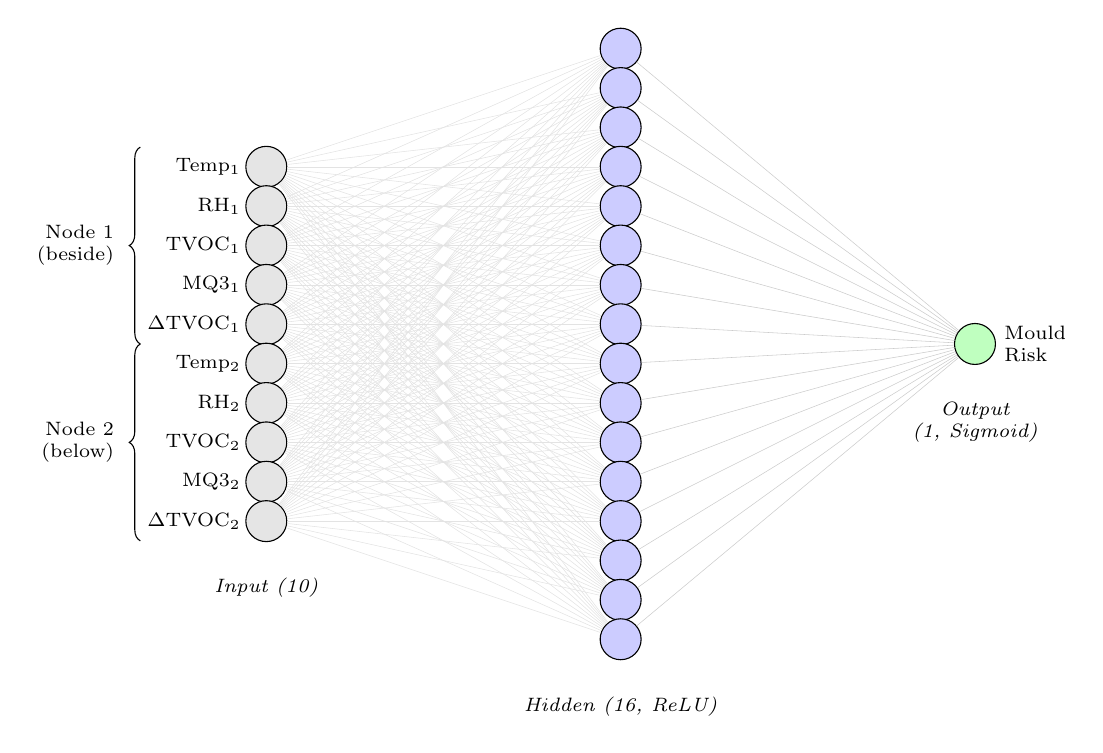
\begin{tikzpicture}[
    inode/.style={circle, draw, fill=gray!20,  minimum size=0.52cm, inner sep=0pt},
    hnode/.style={circle, draw, fill=blue!20,  minimum size=0.52cm, inner sep=0pt},
    onode/.style={circle, draw, fill=green!25, minimum size=0.52cm, inner sep=0pt}
]
% Input layer (10 nodes, 0.5 spacing)
\foreach \i/\y in {1/2.25, 2/1.75, 3/1.25, 4/0.75, 5/0.25,
                   6/-0.25, 7/-0.75, 8/-1.25, 9/-1.75, 10/-2.25}
    \node[inode] (in\i) at (0, \y) {};
% Hidden layer (16 nodes, 0.5 spacing)
\foreach \j/\y in {1/3.75,  2/3.25,  3/2.75,  4/2.25,
                   5/1.75,  6/1.25,  7/0.75,  8/0.25,
                   9/-0.25, 10/-0.75, 11/-1.25, 12/-1.75,
                   13/-2.25, 14/-2.75, 15/-3.25, 16/-3.75}
    \node[hnode] (h\j) at (4.5, \y) {};
% Output node
\node[onode] (out) at (9, 0) {};
% Connections (drawn first, behind nodes)
\foreach \i in {1,...,10}
    \foreach \j in {1,...,16}
        \draw[gray!22, very thin] (in\i) -- (h\j);
\foreach \j in {1,...,16}
    \draw[gray!40, very thin] (h\j) -- (out);
% Input labels (subscript 1 = beside node, subscript 2 = below node)
\node[left=0.2cm, font=\scriptsize] at (in1)  {Temp$_1$};
\node[left=0.2cm, font=\scriptsize] at (in2)  {RH$_1$};
\node[left=0.2cm, font=\scriptsize] at (in3)  {TVOC$_1$};
\node[left=0.2cm, font=\scriptsize] at (in4)  {MQ3$_1$};
\node[left=0.2cm, font=\scriptsize] at (in5)  {$\Delta$TVOC$_1$};
\node[left=0.2cm, font=\scriptsize] at (in6)  {Temp$_2$};
\node[left=0.2cm, font=\scriptsize] at (in7)  {RH$_2$};
\node[left=0.2cm, font=\scriptsize] at (in8)  {TVOC$_2$};
\node[left=0.2cm, font=\scriptsize] at (in9)  {MQ3$_2$};
\node[left=0.2cm, font=\scriptsize] at (in10) {$\Delta$TVOC$_2$};
% Grouping braces
\draw[decorate, decoration={brace, mirror, amplitude=4pt}]
    (-1.6, 2.50) -- (-1.6, 0.0)
    node[midway, left=6pt, font=\scriptsize, align=right] {Node 1\\(beside)};
\draw[decorate, decoration={brace, mirror, amplitude=4pt}]
    (-1.6, 0.0) -- (-1.6, -2.50)
    node[midway, left=6pt, font=\scriptsize, align=right] {Node 2\\(below)};
% Output label
\node[right=0.25cm, font=\scriptsize, align=left] at (out) {Mould\\Risk};
% Layer labels
\node[font=\scriptsize\itshape, align=center] at (0,   -3.1) {Input (10)};
\node[font=\scriptsize\itshape, align=center] at (4.5, -4.6) {Hidden (16, ReLU)};
\node[font=\scriptsize\itshape, align=center] at (9,   -1.0) {Output\\(1, Sigmoid)};
\end{tikzpicture}
\caption{Neural network architecture used across all three TinyML framework variants (193 parameters total). Subscript 1 denotes the node beside the strawberries; subscript 2 denotes the node below the produce level. For TF Lite Micro all weights are frozen post-deployment. For TinyOL the hidden layer is frozen and only the 17 output-layer parameters are updated on-device. For AIfES all 193 weights are trained from scratch on the ESP32.}
\label{fig:nn_architecture}
\end{figure}

\subsection{Dataset}

Data was collected across five separate experimental batches. Batches 1 and 2 formed the primary fit set for the backbone model (AIfES inference and TF Lite Micro). Batch 3 was used exclusively as a validation set for early stopping during backbone training. Batch 4 (287 samples) was deliberately withheld from all backbone training and reserved for TinyOL on-device output-layer fine-tuning. AIfES full on-device training used all available training data --- Batches 1--4 (1278 samples) --- with no held-out validation set. In a real autonomous deployment there would be no infrastructure to support a validation set, and training ran for a fixed 20 epochs regardless of convergence. Batch 5 (332 samples) was withheld as the held-out test set and was never used during any stage of training or validation for any framework, ensuring an uncontaminated evaluation.

\subsection{Feature Engineering}

Raw sensor readings were not passed directly to the network. Each input feature was normalised to the range $[0, 1]$ using min-max scaling fitted on the backbone training set (Batches 1 and 2):

\begin{equation}
    x_{\text{norm}} = \frac{x_{\text{raw}} - x_{\text{min}}}{x_{\text{max}} - x_{\text{min}}}
    \label{eq:minmax}
\end{equation}

The scaling parameters were fixed at training time and embedded in firmware, so the same transformation was applied at inference without any runtime fitting. Values outside the training range were clipped to $[0, 1]$.

In addition to the four raw sensor channels per node (temperature, relative humidity, TVOC, MQ3 ppm), a TVOC rate-of-change feature was computed for each inside node:

\begin{equation}
    \Delta\text{TVOC}[t] = \text{TVOC}[t] - \text{TVOC}[t-1]
    \label{eq:delta_tvoc}
\end{equation}

with $\Delta\text{TVOC}[t] = 0$ for the first reading in each experimental batch. This temporal feature captures whether VOC concentration is actively rising, which is more directly indicative of accelerating fungal metabolic activity than the absolute reading alone. A static elevated-TVOC environment (stable baseline, $\Delta\text{TVOC} \approx 0$) carries different risk information than one in which concentrations are increasing rapidly.

The eCO\textsubscript{2} channel from the SGP30 was collected and transmitted but excluded from the feature set after dataset analysis showed it provided no additional predictive information beyond the TVOC channel, to which it is strongly correlated on this sensor. The master node readings were likewise excluded, as the master was positioned outside the chamber and its readings reflected ambient laboratory conditions rather than the produce environment.

The final feature vector therefore comprises ten values per sample: temperature, relative humidity, TVOC, MQ3 ppm, and $\Delta$TVOC from the beside node ($\times$5) and the below node ($\times$5).

\subsection{TF Lite Micro}

The network was trained offline on a desktop computer using TensorFlow on Batches~1 and~2, with Batch~3 used as a held-out validation set for early stopping. The trained model was post-training quantised to 8-bit integer weights and converted to the \texttt{.tflite} format. The quantised model was embedded in the ESP32 firmware as a constant byte array and loaded into SRAM at runtime. TF Lite Micro performed one forward pass per sensing cycle; no weights were modified after deployment.

\subsection{TinyOL}

The TinyOL configuration used an intentionally weak backbone: the hidden layer was pre-trained on Batch 1 only (approximately 250 samples from a single high-temperature experimental condition), rather than on the full training pool. This was deliberate --- a backbone trained on all batches already generalised well to the test set, leaving no accuracy gap for on-device adaptation to close. By restricting backbone training to a single batch, the model underperformed on the colder, more varied conditions in Batch 5, creating a genuine improvement opportunity for the on-device fine-tuning step.

On-device adaptation used Batch 4 (287 samples) as the fine-tuning dataset. Only the 17 output-layer parameters ($W_2 \in \mathbb{R}^{16}$, $b_2 \in \mathbb{R}$) were updated; the 176 hidden-layer weights remained frozen throughout. The optimiser was stochastic gradient descent (SGD) with a learning rate of 0.001, weighted binary cross-entropy loss, and class weights applied to counteract the 2:1 mould-to-no-mould imbalance in Batch 4. Training ran for 10 epochs with Fisher-Yates shuffling of the fine-tuning dataset before each epoch.

\subsection{AIfES}

For AIfES, no pre-trained weights were used. All 193 network parameters were initialised on the ESP32 using Glorot uniform initialisation and trained entirely on-device. The optimiser was Adam with a learning rate of 0.001 and binary cross-entropy loss. Training ran for 20 epochs over the full training corpus (Batches~1--4, 1278 samples) with no validation set --- consistent with a real autonomous deployment where no labelled holdout would be available. A mini-batch size of 4 was used. A per-epoch Fisher-Yates shuffle was applied to the training data using the ESP32 hardware random number generator.

A batch size of 4 (rather than online stochastic gradient descent with batch size 1) was required to prevent numerical instability: with batch size 1, the Adam squared-gradient accumulator approached zero for near-constant input features, causing division overflow on epoch 20. Averaging the gradients over 4 samples before each parameter update kept the accumulator well away from zero. This is the standard remedy for online Adam instability when gradient clipping is unavailable.

\section{Deployment Model and Battery Lifetime Estimation}\label{sec:deployment_model}

The operational scenario modelled for SQ4 is a duty-cycled node that wakes at 15-minute intervals, completes the SGP30 warm-up, reads all sensors, runs inference (or a scheduled training cycle), and returns to deep sleep. Figure~\ref{fig:duty_cycle} illustrates one complete cycle schematically.

\begin{figure}[htbp]
\centering
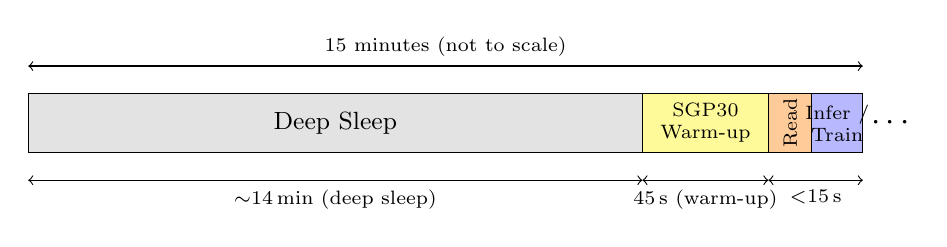
\begin{tikzpicture}
\def\sw{7.8}
\def\wuw{1.6}
\def\sew{0.55}
\def\cw{0.65}
\def\h{0.75}
% Sleep bar
\fill[gray!22] (0,0) rectangle (\sw,\h);
\draw (0,0) rectangle (\sw,\h);
\node[font=\small] at (\sw/2, \h/2) {Deep Sleep};
% Warm-up bar
\fill[yellow!40] (\sw,0) rectangle (\sw+\wuw,\h);
\draw (\sw,0) rectangle (\sw+\wuw,\h);
\node[font=\scriptsize, align=center] at (\sw+\wuw/2, \h/2) {SGP30\\Warm-up};
% Sense bar
\fill[orange!40] (\sw+\wuw,0) rectangle (\sw+\wuw+\sew,\h);
\draw (\sw+\wuw,0) rectangle (\sw+\wuw+\sew,\h);
\node[font=\scriptsize, align=center, rotate=90] at (\sw+\wuw+\sew/2, \h/2) {Read};
% Compute bar
\fill[blue!28] (\sw+\wuw+\sew,0) rectangle (\sw+\wuw+\sew+\cw,\h);
\draw (\sw+\wuw+\sew,0) rectangle (\sw+\wuw+\sew+\cw,\h);
\node[font=\scriptsize, align=center] at (\sw+\wuw+\sew+\cw/2, \h/2) {Infer /\\Train};
% Continuation
\node[font=\large] at (\sw+\wuw+\sew+\cw+0.35, \h/2) {$\cdots$};
% Cycle bracket
\draw[<->] (0, \h+0.35) -- (\sw+\wuw+\sew+\cw, \h+0.35)
    node[midway, above, font=\scriptsize] {15 minutes (not to scale)};
% Duration labels
\draw[<->] (0,-0.35) -- (\sw,-0.35)
    node[midway, below, font=\scriptsize] {$\sim$14\,min (deep sleep)};
\draw[<->] (\sw,-0.35) -- (\sw+\wuw,-0.35)
    node[midway, below, font=\scriptsize] {45\,s (warm-up)};
\draw[<->] (\sw+\wuw,-0.35) -- (\sw+\wuw+\sew+\cw,-0.35)
    node[midway, below, font=\scriptsize] {$<$15\,s};
\end{tikzpicture}
\caption{Schematic duty cycle for one 15-minute sampling interval (not to scale). The SGP30 warm-up phase at 45\,s dominates the active window. For AIfES, a training cycle replaces inference once every 24 hours.}
\label{fig:duty_cycle}
\end{figure}

Battery lifetime was estimated analytically from the measured per-phase current consumption figures. For a battery of capacity $Q$ (in \si{\milli\ampere\hour}), estimated runtime $T$ in hours is:

\begin{equation}
    T = \frac{Q}{I_{\text{avg}}}
    \label{eq:battery_lifetime}
\end{equation}

where $I_{\text{avg}}$ is the average current over one complete 15-minute cycle, computed as the time-weighted mean across all operational phases:

\begin{equation}
    I_{\text{avg}} = \frac{\displaystyle\sum_{i} I_i \cdot t_i}{\displaystyle\sum_{i} t_i}
    \label{eq:avg_current}
\end{equation}

with $I_i$ and $t_i$ denoting the mean current and duration of phase $i$ respectively. Two hardware configurations were modelled: the measured prototype with the MQ3, and an improved configuration in which the MQ3 is replaced by a lower-power MEMS gas sensor. The MQ3's continuous \SI{103.3}{\milli\ampere} per-node heater current dominates the power budget; the improved configuration was modelled analytically from published datasheet figures for a representative MEMS alternative rather than measured directly.
